\chapter{Konzept}
\label{chapter_Konzept}

Im folgenden Kapitel wird auf die Erstellung des Konzeptes eingegangen.

\section{Teststand}
\label{section_Teststand}

Das Gesamtsystem setzt sich aus drei Untersystemen zusammen:

\begin{itemize}

\item Mess-Client
\begin{itemize}
\item Übernimmt die lokale Ansteuerung der \acp{DUT}
\item Nimmt Messdaten auf und stellt sie zur Verfügung
\end{itemize}

\item Mess-Server
\begin{itemize}
\item Verwaltet angeschlossene Mess-Clients
\item Speichert alle Messdaten
\item Bildet das Bindeglied zwischen Mess-Client und dem PC-Client
\end{itemize}

\item PC-Client
\begin{itemize}
\item Parametriert die Mess-Clients
\item Wertet Messdaten aus und stellt sie leserlich da
\end{itemize}

\end{itemize}


\begin{figure}[H]
\begin{center}
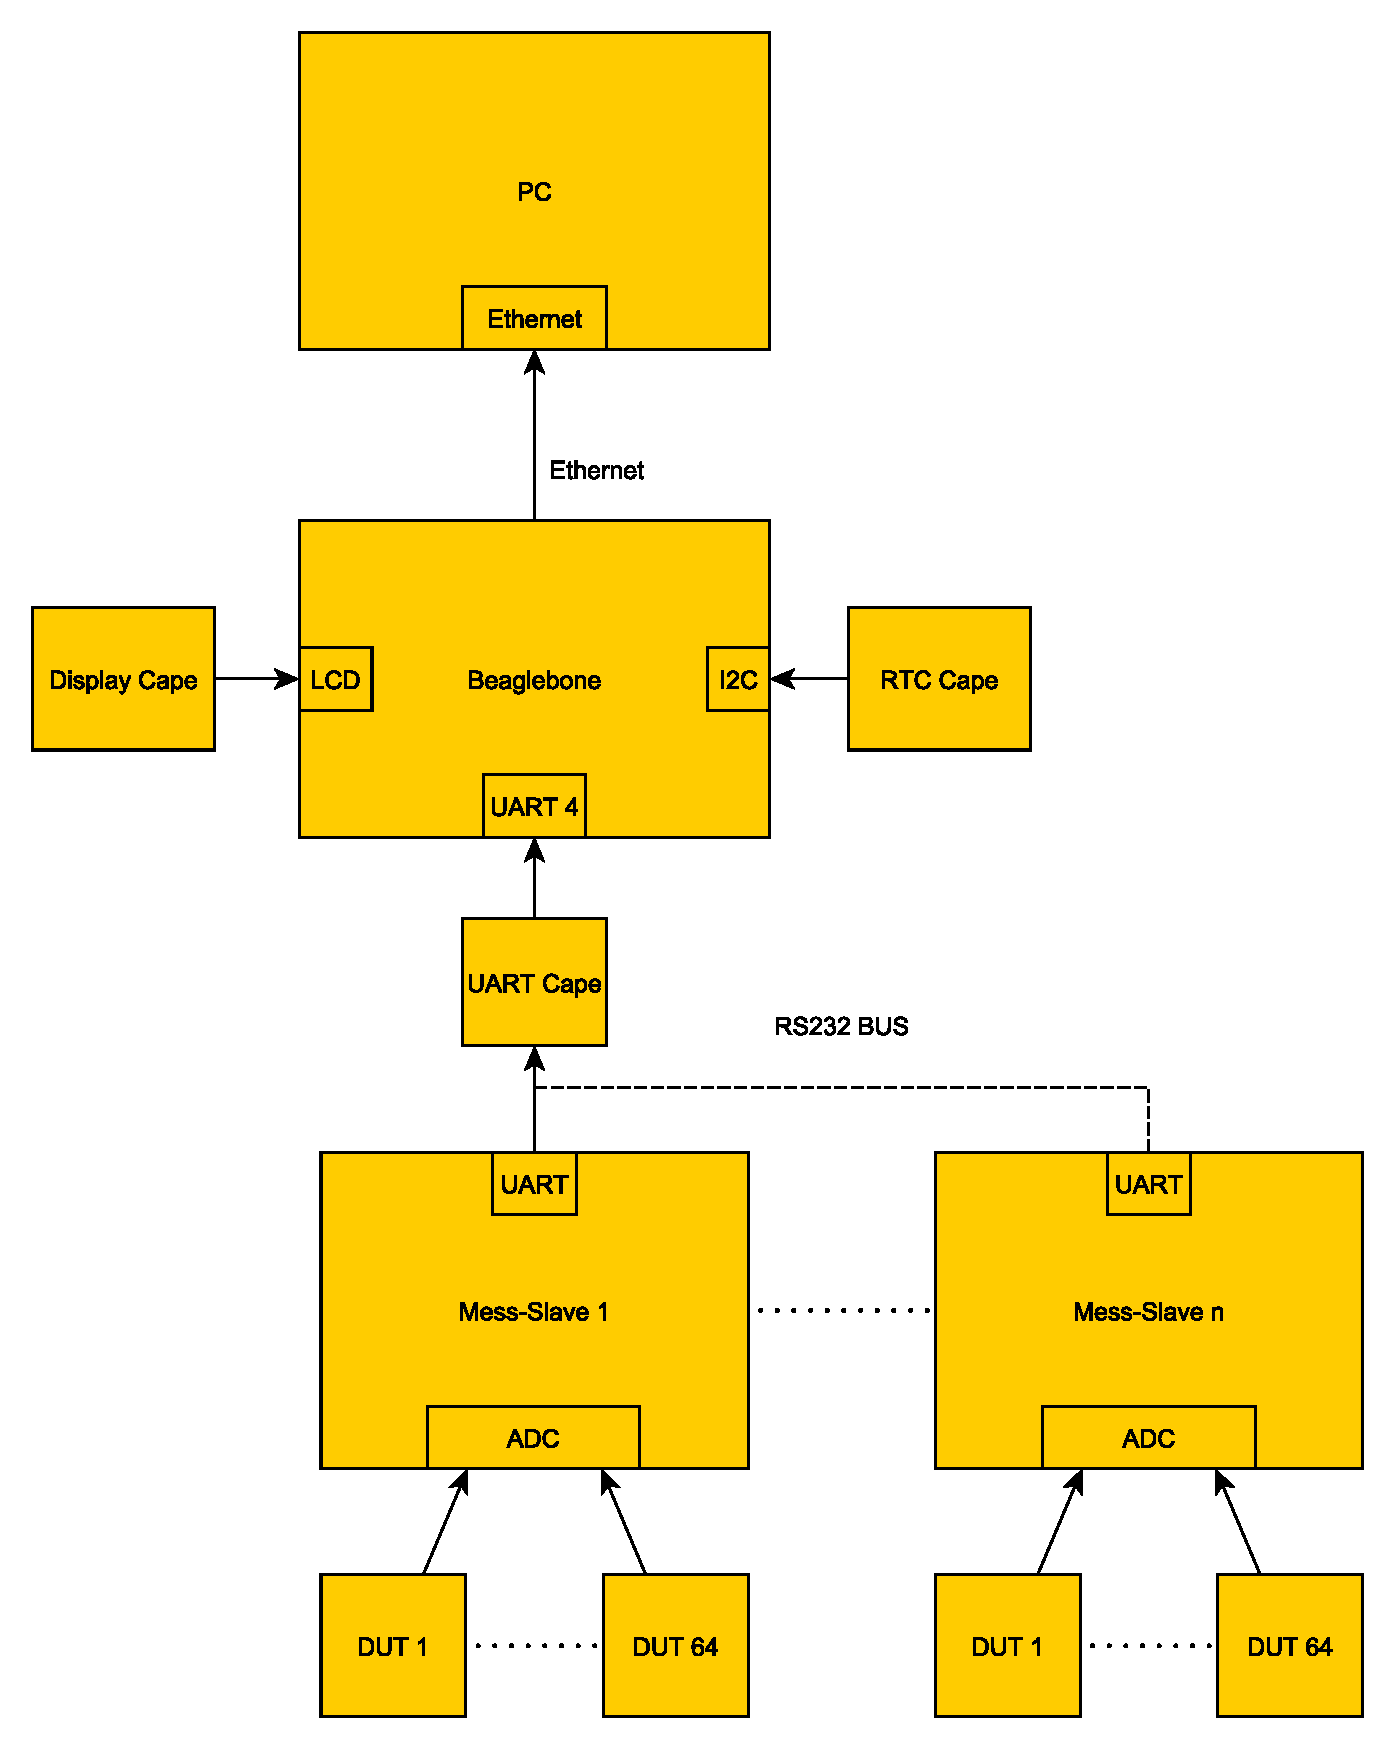
\includegraphics[width=\textwidth]{img/general/BlockPlan.pdf}
\caption{Gesamt System}
\label{Gesamt_System}
\end{center}
\end{figure}


\subsection{Mess-Client}
\label{section_Mess-Client}

Das Herzstück des Mess-Clients bildet ein STM8  8-Bit Mikrocontroller der Firma STMicroelectronics.
Auf jedem Mess-Client sind 64 \acp{DUT} befestigt. In zyklischen Abständen werden die Messdaten der Prüfobjekte aufgenommen und über eine RS232-Schnittstelle zur Verfügung gestellt (siehe Abbildung \ref{MessSlaveBlockPlan}.\\
Dieses System war zum großen Teil bereits gegeben, so dass lediglich die Übertragung der RS232 Schnittstelle geregelt werden musste. Dazu wurde ein Protokoll für die Kommunikation entworfen (sieht Abschnitt \ref{section_RS232_Protokoll}).
\\
%\begin{figure}[h]
%\begin{center}
%\includegraphics[width=\textwidth]{}
%\caption{Mess-Client Blockschaltplan}
%\label{MessSlaveBlockPlan}
%\end{center}
%\end{figure}


\subsection{Mess-Server}
\label{section_Mess-Server}

Als Mess-Server wird ein BeagleBone Black von Texas Instruments eingesetzt. Dabei handelt es sich um einen Einplatinen-Computer, der mit einem AM335x 1GHz ARM® Cortex-A8 Prozessor arbeitet. Das Betriebssystem ist eine Embedded Linux Debian Lösung.


\subsection{PC-Client}
\label{section_Verwaltung}
asdasad


\subsection{RS232 Protokoll}
\label{section_RS232_Protokoll}
Das Protokoll für die Kommunikation über die RS232 Schnittstelle ist nötig, um die Validität, Vollständigkeit und Zuverlässigkeit der Übertragungen sicherzustellen.\ \\

Folgende Kriterien sollen dabei erfüllt werden:
\begin{itemize}
\item Adressierung individueller Kommunikationspartner
\item Senden verschiedener Befehle
\item Variable Größe der Daten
\item Sicherstellung der Validität der Übertragung
\item Erweiterbar
\end{itemize}
\ \\

\subsubsection{Aufbau}
\begin{table}[H]
\begin{center}
\begin{tabularx}{\textwidth}{|X|X|X|X|c|X|}\hline
 1. Byte & 2. Byte & 3. Byte & 4. Byte & 5. Byte und folgend & Letztes Byte\\ \hline
  Adresse & Länge & Command & Subcommand & Nutzdaten & Checksumme\\ \hline
\end{tabularx}
\caption{Übertragungsrahmen}
\label{table_Frame}
\end{center}
\end{table}

Ein Rahmen besteht aus 4 Steuerbytes, 1 Checksummenbyte und maximal 30 Datenbytes. 

\textbf{1. Byte: Adresse \& Read/Write}

\begin{table}[H]
\begin{center}
\begin{tabularx}{\textwidth}{|X|X|X|X|X|X|X|X|}\hline
 7. Bit & 6. Bit & 5. Bit & 4. Bit & 3. Bit & 2. Bit & 1. Bit & 0. Bit\\ \hline
 R/W & Addr6 & Addr5 & Addr4 & Addr3 & Addr2 & Addr1 & Addr0\\ \hline
\end{tabularx}
\caption{1. Byte: Adresse \& Read/Write}
\label{table_1Byte}
\end{center}
\end{table}

Das erste Byte des Übertragungsrahmens setzt sich aus 7 Adressbits und einem Lese-/Schreibbit zusammen. Die ersten 7 Bits (Addr0 - Addr6) bilden die Adresse des anzusteuernden Mess-Clients. Daraus ergibt sich ein Adressraum von möglichen 128 Adressen, wobei Adresse 0 für neue Mess-Clients zur einmaligen Anmeldung im System reserviert ist.\\
Das höchste Bit ist das Lese-/Schreibbit. Der Mess-Client unterscheidet mithilfe dieses Bits, ob ein Befehl als Lese- oder Schreibzugriff interpretiert werden soll.\\

\begin{table}[H]
\begin{center}
\begin{tabular}{|l|l|}\hline
 R/W Bit & Beschreibung \\ \hline
 0 & Die Steuereinheit möchte lesen \\ \hline
 1 & Die Steuereinheit möchte schreiben \\ \hline
\end{tabular}
\caption{Read/Write}
\label{table_RW}
\end{center}
\end{table}


\textbf{2. Byte: Länge des Rahmens}

\begin{table}[H]
\begin{center}
\begin{tabularx}{\textwidth}{|X|X|X|X|X|X|X|X|}\hline
 7. Bit & 6. Bit & 5. Bit & 4. Bit & 3. Bit & 2. Bit & 1. Bit & 0. Bit\\ \hline
 Len7 & Len6 & Len5 & Len4 & Len3 & Len2 & Len1 & Len0\\ \hline
\end{tabularx}
\caption{2. Byte: Länge des Rahmens}
\label{table_2Byte}
\end{center}
\end{table}

Das zweite Byte gibt die Länge des gesamten Übertragungsrahmens inklusive Steuerbytes, Nutzdaten und Checksumme an.\\ Die minimale Länge eines Rahmens beträgt 5 Byte. Dabei handelt es sich um eine Übertragung ohne Nutzdaten und es werden lediglich die 4 Steuerbytes und das Byte für die Checksumme übertragen. Dies geschieht beispielsweise bei einer Leseanfrage.\\
Die maximale Länge eines Rahmen beträgt 35 Byte. Hierbei werden zusätzlich zu den 4 Steuerbytes und dem Byte für die Checksumme auch die maximale Nutzlast von 30 Byte übertragen. Dieser Fall kann beispielsweise bei Schreibzugriffen auftreten.


\textbf{3. Byte: Command}

\begin{table}[H]
\begin{center}
\begin{tabularx}{\textwidth}{|X|X|X|X|X|X|X|X|}\hline
 7. Bit & 6. Bit & 5. Bit & 4. Bit & 3. Bit & 2. Bit & 1. Bit & 0. Bit\\ \hline
 Cmd7 & Cmd6 & Cmd5 & Cmd4 & Cmd3 & Cmd2 & Cmd1 & Cmd0\\ \hline
\end{tabularx}
\caption{3. Byte: Command}
\label{table_3Byte}
\end{center}
\end{table}

Das dritte Byte repräsentiert den Befehl. Dieser gibt an, welche Aktion ausgeführt werden soll oder welcher Parameter angesprochen wird. 


\textbf{4. Byte: Subcommand}

\begin{table}[H]
\begin{center}
\begin{tabularx}{\textwidth}{|X|X|X|X|X|X|X|X|}\hline
 7. Bit & 6. Bit & 5. Bit & 4. Bit & 3. Bit & 2. Bit & 1. Bit & 0. Bit\\ \hline
 Scmd7 & Scmd6 & Scmd5 & Scmd4 & Scmd3 & Scmd2 & Scmd1 & Scmd0\\ \hline
\end{tabularx}
\caption{4. Byte: Subcommand}
\label{table_4Byte}
\end{center}
\end{table}

Das vierte Byte ist der Subcommand. Damit ist es möglich verschiedene Unterbefehle zu adressieren.


\textbf{5. Byte und folgend: Nutzdaten}

\begin{table}[H]
\begin{center}
\begin{tabularx}{\textwidth}{|X|X|X|X|X|X|X|X|}\hline
 7. Bit & 6. Bit & 5. Bit & 4. Bit & 3. Bit & 2. Bit & 1. Bit & 0. Bit\\ \hline
 Data7 & Data6 & Data5 & Data4 & Data3 & Data2 & Data1 & Data0\\ \hline
\end{tabularx}
\caption{5. Byte und folgend: Nutzdaten}
\label{table_5Byte}
\end{center}
\end{table}

Das fünfte Byte und die darauf folgendenx, tragen die Nutzdaten des Rahmens. 


\textbf{Letztes Byte: Checksumme}

\begin{table}[H]
\begin{center}
\begin{tabularx}{\textwidth}{|X|X|X|X|X|X|X|X|}\hline
 7. Bit & 6. Bit & 5. Bit & 4. Bit & 3. Bit & 2. Bit & 1. Bit & 0. Bit\\ \hline
 CKS7 & CKS6 & CKS5 & CKS4 & CKS3 & CKS2 & CKS1 & CKS0\\ \hline
\end{tabularx}
\caption{Letztes Byte: Checksumme}
\label{table_LastByte}
\end{center}
\end{table}

Das letzte Byte ist immer die Checksumme um sicherzustellen, dass alle Daten komplett und fehlerfrei übertragen wurden. Die Checksumme bildet sich dabei aus einer XOR Verknüpfung aller Bytes eines Übertragungsrahmens.

Beispiel:

Checksumme bilden:
 
1 xor 2 xor 3 xor 4 xor 5 = 1

Checksumme prüfen:

1 xor 2 xor 3 xor 4 xor 5 xor 1 = 0

\subsubsection{Commands und Subcommands}


\begin{table}[H]
\begin{center}
\begin{tabularx}{\textwidth}{|l|c|c|c|X|}\hline
 Command & Code & Subcommand & Datenbytes & Content Datatype\\ \hline
 ADC-Value & 0x00 & MUX-Kanal (0..63) & 2 & ADC Wert für spezifizierten Kanal \\ \hline
 Number Of Pulses & 0x04 & - & 1 & Anzahl der Pulse pro Pattern (0..50) \\ \hline
 Pulsewidth and -period & 0x05 & Pulsnummer & 4 & Pulsbreite und Pulseperiode \\ \hline
 Perform Pulseupdate & 0x06 & - & 0 &  \\ \hline
 DAC-value & 0x07 & - & 2 & DAC Wert \\ \hline
 Temperature & 0x08 & - & 1 & Wert des Temperatursensors \\ \hline
 LTT name & 0x09 & - & 1..30 & Name \\ \hline
 Rs232-Address & 0x0A & - & 1 & Adresse \\ \hline
 Error & 0x0B & MUX-Channel (0..63) & 2 & ADC Value for specified Channel \\ \hline
 Measurement Intervall & 0x0C & Intervallnummer (0..2) & 4 & Minutenabstand zwischen den Messungen + Tagesabstand zum nächsten Interval \\ \hline
\end{tabularx}
\caption{Befehlsliste}
\label{table_Commands}
\end{center}
\end{table}



\section{Datenbank}
\label{section_EntwurfDatenbank}

Aus den Anforderungen ergibt sich folgendes \ac{ERM} (siehe Abbildung \ref{ERM}). \\

\begin{figure}[H]
\begin{center}
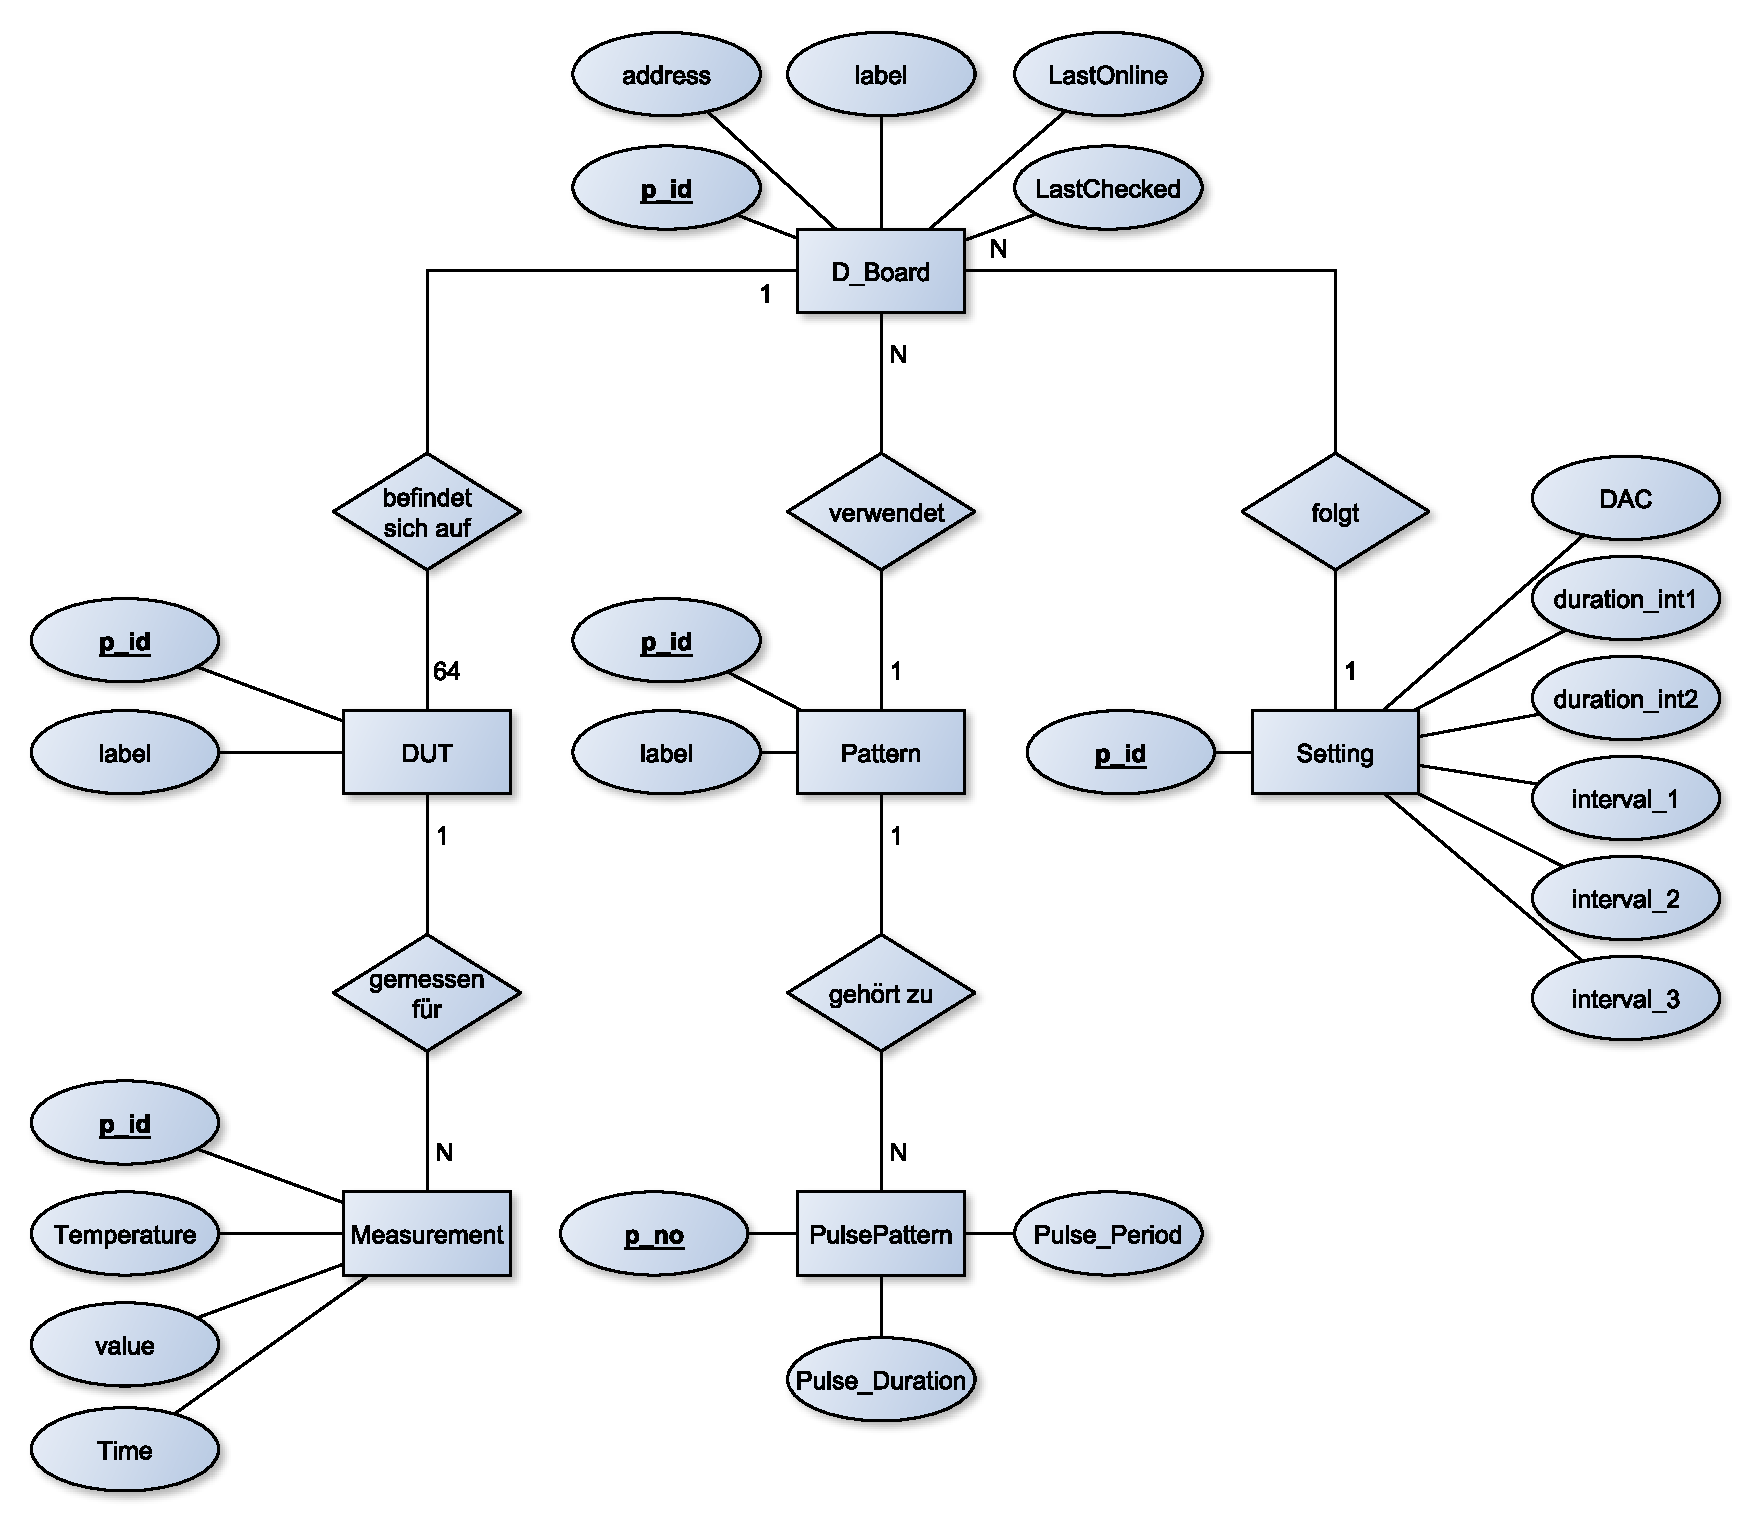
\includegraphics[width=\textwidth]{img/general/ER_Diagramm.pdf}
\caption{Entity Relationship Modell}
\label{ERM}
\end{center}
\end{figure}


Die Datenbank muss folgende Daten für die Parameter der Mess-Clients aufnehmen:\\

\begin{table}[H]
\begin{center}
\begin{tabular}{|l|l|}\hline
Parameter & Beschreibung \\ \hline
DAC & Vorverstärkung\\ 
duration\_int1 & Dauer der Zeit die Werte im 1.Interval aufgenommen werden in Tagen\\ 
duration\_int2 & Dauer der Zeit die Werte im 2.Interval aufgenommen werden in Tagen\\ 
interval\_1 & Abstand zwischen den Messungen im 1. Interval in Minuten\\ 
interval\_2 & Abstand zwischen den Messungen im 2. Interval in Minuten\\ 
interval\_3 & Abstand zwischen den Messungen nach dem 2. Interval in Minuten\\ \hline
\end{tabular}
\caption{Tabelle Setting}
\label{table_TabelleSetting}
\end{center}
\end{table}




